\documentclass[11pt]{article}
\usepackage[review]{acl}
\usepackage{times}
\usepackage{latexsym}
\usepackage[T1]{fontenc}
\usepackage[utf8]{inputenc}
\usepackage{microtype}
\usepackage{inconsolata}
\usepackage{graphicx}
\usepackage{booktabs}
\usepackage{multirow}
\usepackage{amsmath}
\usepackage{amssymb}
\usepackage{array}
\usepackage{enumitem}
\usepackage{xspace}
\usepackage{xcolor}
\usepackage{adjustbox}

\newcommand{\bench}{ClinSemBench\xspace}
\newcommand{\Pc}{\textsc{p}\xspace}
\newcommand{\Cc}{\textsc{c}\xspace}
\newcommand{\ctrlz}{\textsc{Ctrl-0}\xspace}
\newcommand{\ctrlo}{\textsc{Ctrl-1}\xspace}
\newcommand{\ctrlt}{\textsc{Ctrl-2}\xspace}
\newcommand{\confr}{\textsc{Conf-R}\xspace}
\newcommand{\confp}{\textsc{Conf-P}\xspace}
\newcommand{\tbd}[1]{\textcolor{red}{[TBD: #1]}}
\newcommand{\chg}[1]{\textbf{#1}}

\title{Surface or Semantics? Disentangling What Radiology Report Metrics Measure with Factorial Minimal Pairs}

\author{Anonymous ACL submission}

\begin{document}
\maketitle

\begin{abstract}
Metrics for radiology report generation are increasingly validated with perturbation suites: a reference report is edited so that its meaning is either preserved or changed, and a good metric should penalise the second kind of edit more.
We show that this protocol confounds two things.
In existing suites the two kinds of edit differ systematically in how much surface text they change, so the label can be predicted without reading the meaning: a classifier that sees only surface statistics reaches an AUROC of 0.92--0.96 on a recent suite and 0.83 on its human-validated subset.
Worse, the direction of the confound depends on how the meaning-preserving edits were built, so the same metric can look sensitive in one suite and inverted in another.
We introduce \bench, a factorial minimal-pair benchmark over IU X-Ray and MIMIC-CXR in which each target sentence receives a meaning-preserving and a meaning-changing edit at the same position with matched surface form, crossed with three levels of surrounding surface noise.
Controlling the surface changes the conclusions.
A widely reported ``reversal'' of BERTScore disappears (paired accuracy 0.00 $\rightarrow$ 0.63--0.66); RadGraph F1, F1CheXbert and a temporal metric do not beat a meaning-blind token-overlap baseline; GREEN loses 8--9 points when the surrounding sentences are paraphrased while CRIMSON does not.
In a monotonicity test with fixed surface, metrics that look perfectly monotone under the usual ``more errors, more edits'' ladder drop to Kendall $\tau \le 0.2$.
Strong reasoning LLM judges reach 0.95--0.97 but still miss certainty changes under paraphrase and are prompt-sensitive.
We recommend reporting a meaning-blind baseline and a surface-only predictability score with every perturbation-based meta-evaluation.
\end{abstract}

\section{Introduction}

Automatic radiology report generation is evaluated almost entirely by comparing a generated report with a reference, and the metric used for that comparison decides which systems appear to make progress.
Because report text carries clinical statements, a metric should ignore harmless rewording and react to statements that differ: ``No pleural effusion'' and ``Pleural effusion is not seen'' say the same thing, while ``Small left pleural effusion'' and ``Small right pleural effusion'' do not.

A growing line of work tests metrics for exactly this property with \emph{perturbation suites}.
A reference report is edited in a controlled way; some edits are meant to preserve its meaning and some to change it; a metric is credited when it penalises the meaning-changing edits more \citep{sai-etal-2021-perturbation,ribeiro-etal-2020-beyond,reevalmed-2025,radsem-2026}.
The protocol is attractive: labels come for free and failures can be attributed to a kind of edit.

This paper starts from an uncomfortable observation about our own earlier suite of this kind.
A token-set overlap score (Jaccard), which has no access to meaning, separated its meaning-changing from its meaning-preserving candidates as well as the best LLM-based metric did, on rule labels and on human labels alike.
The reason is mundane.
The meaning-preserving edits (reformatting, sentence reordering) rewrote many tokens but left the bag of tokens intact; the meaning-changing edits replaced one word.
A metric could therefore earn a high score by counting changed tokens, and a metric that is proportional to edit size, such as BERTScore, was reported as ``directionally reversed''.
Neither result says much about semantics.

The problem is not specific to that suite.
When meaning-preserving candidates are produced by free rewriting and meaning-changing ones by local error injection, the confound points the other way: overlap-based metrics now score the erroneous candidates \emph{higher}, a pattern visible in published per-metric averages \citep{reevalmed-2025}.
The same metric can thus look sensitive or inverted depending on how the benign edits were constructed (\S\ref{sec:diagnosis}).
As with annotation artifacts in NLI \citep{gururangan-etal-2018-annotation,mccoy-etal-2019-right}, the test can be passed for the wrong reason.

We address the confound by design.
\bench builds, for one target sentence of a report section, a meaning-preserving edit (\Pc) and a meaning-changing edit (\Cc) \emph{at the same position and with the same surface operation}, so that the two candidates are equally far from the reference on the surface and differ only in the meaning slot (Figure~\ref{fig:design}).
This pair is then crossed with three levels of surface noise in the rest of the section: none, sentence reordering, and paraphrase of all other sentences.
Comparing \Cc with \Pc inside one level gives a controlled test; comparing a minimally edited \Cc with a heavily rewritten \Pc reproduces, inside a single dataset and with identical targets, the confounds of existing suites in both directions.

Our contributions are:
\begin{enumerate}[leftmargin=*,noitemsep]
\item \textbf{A diagnosis.} Labels of existing perturbation suites are predictable from surface statistics alone, and the direction of the resulting confound depends on the construction of the benign edits. We propose two cheap controls for any such suite: a meaning-blind baseline and a surface-only predictability score.
\item \textbf{A design.} A factorial minimal-pair benchmark on two chest X-ray corpora (1,940 targets, seven edit types, six cells per target) with position- and shape-matched edits, plus a fixed-surface monotonicity set. In the controlled cells a surface-only classifier is near chance (0.52--0.64 AUROC against 0.98--1.00 in the confounded ones).
\item \textbf{Findings that change under control.} For 15 metrics and six LLM judges we separate sensitivity to meaning from sensitivity to surface. Several conclusions drawn from confounded suites do not survive, including the BERTScore reversal and the apparent monotonicity of overlap and graph metrics; others emerge only under control, such as GREEN's degradation under paraphrase, clinical metrics that fail to beat token overlap, and the non-monotone behaviour of rubric-style LLM judges.
\end{enumerate}

\begin{figure*}[t]
\centering
\small
\setlength{\tabcolsep}{4pt}
\begin{tabular}{p{0.085\textwidth}p{0.42\textwidth}p{0.42\textwidth}}
\toprule
 & \textbf{\Pc: meaning-preserving} & \textbf{\Cc: meaning-changing} \\
\midrule
\textbf{S0} minimal &
\textbf{P0}\; The heart is normal in size. The pulmonary vascularity is within normal limits in appearance. No pneumothorax or pleural effusion. Patchy \chg{right-sided} lower lung opacification is noted. &
\textbf{C0}\; The heart is normal in size. The pulmonary vascularity is within normal limits in appearance. No pneumothorax or pleural effusion. Patchy \chg{left-sided} lower lung opacification is noted. \\
\addlinespace
\textbf{S1} reorder &
\textbf{P1}\; Patchy \chg{right-sided} lower lung opacification is noted. The heart is normal in size. The pulmonary vascularity is within normal limits in appearance. No pneumothorax or pleural effusion. &
\textbf{C1}\; Patchy \chg{left-sided} lower lung opacification is noted. The heart is normal in size. The pulmonary vascularity is within normal limits in appearance. No pneumothorax or pleural effusion. \\
\addlinespace
\textbf{S2} paraphrase &
\textbf{P2}\; The size of the heart is within normal limits. The appearance of the pulmonary vascularity is within normal limits. No pleural effusion or pneumothorax. Patchy \chg{right-sided} lower lung opacification is noted. &
\textbf{C2}\; The size of the heart is within normal limits. The appearance of the pulmonary vascularity is within normal limits. No pleural effusion or pneumothorax. Patchy \chg{left-sided} lower lung opacification is noted. \\
\bottomrule
\end{tabular}
\caption{The six cells built from one target (IU X-Ray; edit type \emph{laterality}). Reference: ``The heart is normal in size. The pulmonary vascularity is within normal limits in appearance. No pneumothorax or pleural effusion. Patchy \chg{right} lower lung opacification is noted.'' Within a row, \Pc and \Cc apply the same surface operation at the same position and differ only in the side. \emph{Controlled} comparisons stay within a row (\ctrlz: C0 vs.\ P0; \ctrlo; \ctrlt). \emph{Confounded} comparisons cross rows: \confr (C0 vs.\ P1) mimics suites whose benign edits reorder or reformat text; \confp (C0 vs.\ P2) mimics suites whose benign edits are free rewrites.}
\label{fig:design}
\end{figure*}

\section{Related Work}

\paragraph{Metrics for radiology reports.}
Beyond BLEU \citep{papineni-etal-2002-bleu}, ROUGE \citep{lin-2004-rouge} and BERTScore \citep{zhang-etal-2020-bertscore}, the field uses label-based scores built on CheXbert \citep{smit-etal-2020-chexbert}, entity--relation overlap from RadGraph \citep{jain-etal-2021-radgraph}, the composite RadCliQ \citep{yu-etal-2023-evaluating}, the entity-aware RaTEScore \citep{zhao-etal-2024-ratescore}, structured-report classifiers \citep{delbrouck-etal-2025-srr}, temporal-entity scores \citep{zhang-etal-2025-libra}, and LLM-based metrics that enumerate errors, such as GREEN \citep{ostmeier-etal-2024-green}, FineRadScore \citep{huang-etal-2024-fineradscore} and CRIMSON \citep{crimson-2026}. Many are packaged in RadEval \citep{xu-etal-2025-radeval}, which we use.

\paragraph{Meta-evaluation with perturbations.}
Behavioural testing \citep{ribeiro-etal-2020-beyond} and perturbation checklists for generation metrics \citep{sai-etal-2021-perturbation} motivate suites for radiology. ReEvalMed \citep{reevalmed-2025} has an LLM rewrite reports along one aspect at a time, with clinician validation, and scores metrics on discrimination, robustness and monotonicity. Its authors note that their clinically insignificant rewrites change more surface text than the significant ones, but do not control for it; \citet{beyond-scalar-2026} evaluate LLM judges on the same data and report that they over-penalise harmless rewrites. RadSEM \citep{radsem-2026} builds a multi-level monotonicity test and uses synonym substitution to reduce lexical artifacts; RadOT-Eval \citep{radot-2026} adds a count-only control baseline to an error-injection stress test; \citet{reref-2026} show that metrics are sensitive to reporting-practice differences between equally valid references. We contribute the quantification of the surface confound, a design that removes it, and evidence that conclusions change when it is removed. Our question about LLM judges is correspondingly narrower than in prior work: do false alarms on harmless rewrites remain once the rewrite is as small as the error it is compared with?

\paragraph{Shortcuts and contrast sets.}
That a benchmark can be solved from superficial cues is well documented for NLI \citep{gururangan-etal-2018-annotation,mccoy-etal-2019-right}; contrast sets \citep{gardner-etal-2020-evaluating} and counterfactual augmentation \citep{kaushik-etal-2020-learning} respond with minimally different inputs whose labels differ. Our matched \Pc/\Cc pairs are contrast sets for metrics, with the additional requirement that the two members be equidistant from a third text, the reference.

\section{Diagnosis: Labels Are Predictable from Surface Alone}
\label{sec:diagnosis}

\paragraph{A surface-only probe.}
For a (reference, candidate) pair we compute ten features that do not depend on meaning: drops in Jaccard and token-F1 overlap, word- and character-level sequence-match ratios, the number and fraction of edited tokens, the length ratio and absolute length difference, whether the bag of tokens changed, and whether any number changed. A logistic regression on these features is trained to predict whether the candidate is labelled meaning-changing, with five-fold cross-validation grouped by report. An AUROC of 0.5 means the label carries no surface signal. We also report the AUROC of two single features.

\paragraph{An existing suite.}
We apply the probe to the suite of our earlier submission, which edits MIMIC-CXR sections with twelve rules (three meaning-preserving: reformatting, sentence reordering, a fixed paraphrase; nine meaning-changing) and includes 467 pairs with adjudicated human labels.
Table~\ref{tab:surface} (top) shows that the probe reaches 0.92 and 0.96 on rule labels and 0.83 on human labels.
For comparison, the best metric in that study, GREEN, reached 0.90 on rule labels and 0.81 on human labels.
Two opposite single-feature cues coexist: candidates whose token bag changed are meaning-changing (Jaccard 0.81--0.89), and candidates with many edited tokens are meaning-preserving (edit count 0.16--0.24).
A metric aligned with the first cue looks sensitive; one aligned with the second looks inverted.

\paragraph{The direction depends on construction.}
ReEvalMed's data are not public, but its reported averages are informative: BLEU, ROUGE-L, RadGraph and BERTScore all assign \emph{higher} mean scores to candidates with clinically significant errors than to clinically insignificant rewrites (e.g.\ BLEU 78.5 vs.\ 41.9), while GREEN does not separate the two groups (74.3 vs.\ 74.8).
Here benign rewrites change the bag of tokens, so only the ``large edit means benign'' cue remains and overlap metrics appear inverted.
We reproduce both regimes inside \bench by choosing which benign cell a minimally edited \Cc is compared with (Table~\ref{tab:surface}, \confr and \confp): the probe reaches 0.98--1.00 in both, while Jaccard alone flips from 0.56--0.59 to 0.01--0.05.
In the controlled cells the probe falls to 0.52--0.54 (\ctrlt) and 0.62--0.64 (\ctrlz).

\begin{table}[t]
\centering
\scriptsize
\setlength{\tabcolsep}{2.5pt}
\begin{adjustbox}{max width=\columnwidth}
\begin{tabular}{lrccc}
\toprule
\textbf{Benchmark / comparison} & \textbf{$n$} & \textbf{Surface-only} & \textbf{Jaccard} & \textbf{\#Edit tok.} \\
\midrule
ClinSemBench-v1, \textit{Impression} (rule labels) & 2,400 & 0.92 & 0.85 & 0.19 \\
ClinSemBench-v1, \textit{Findings} (rule labels) & 2,400 & 0.96 & 0.89 & 0.16 \\
ClinSemBench-v1, validation set (human labels) & 467 & 0.83 & 0.81 & 0.24 \\
RaTE-Eval, synthetic task (synonym vs.\ opposite)$^{\dagger}$ & 1,478 & 0.89 & 0.17 & 0.21 \\
\midrule
Ours, \textsc{Conf-R}: C0 vs.\ P1 & 1,780/2,100 & 1.00/1.00 & 0.59/0.56 & 0.00/0.00 \\
Ours, \textsc{Conf-P}: C0 vs.\ P2 & 1,780/2,100 & 0.98/1.00 & 0.05/0.01 & 0.02/0.00 \\
Ours, \textsc{Ctrl-0}: C0 vs.\ P0 & 1,780/2,100 & 0.64/0.62 & 0.59/0.56 & 0.51/0.51 \\
Ours, \textsc{Ctrl-2}: C2 vs.\ P2 & 1,780/2,100 & 0.54/0.52 & 0.52/0.51 & 0.50/0.50 \\
\bottomrule
\end{tabular}
\end{adjustbox}
\caption{AUROC for predicting the meaning-changing label from surface statistics only. \emph{Surface-only}: cross-validated logistic regression on ten surface features. \emph{Jaccard}, \emph{\#Edit tok.}: single features. Values far from 0.5 in either direction mean the label leaks through surface form.}
\label{tab:surface}
\end{table}

\section{\bench: Factorial Minimal Pairs}
\label{sec:design}

\subsection{Cells and Comparisons}

Let $x$ be a reference section with sentences $s_1,\dots,s_n$ ($n\ge3$) and $s_k$ a target sentence. A rule produces two rewrites of $s_k$: $p$ (meaning-preserving) and $c$ (meaning-changing). The six candidates of Figure~\ref{fig:design} replace $s_k$ by $p$ or $c$ and apply one of three operations to the other sentences: none (S0), a random permutation of all sentences shared by both candidates (S1), or paraphrase of every non-target sentence, again shared (S2). On average \Pc and \Cc edit 4--6\% of the tokens of the reference in S0, while S1 and S2 displace 75--77\% and 60--65\%.

For a metric $m$ oriented so that higher means closer to the reference, the penalty of candidate $\tilde{x}$ is $\Delta_m(\tilde{x}) = m(x,x) - m(x,\tilde{x})$. Our main statistic is \emph{paired accuracy}: the share of targets for which $\Delta_m(\Cc) > \Delta_m(\Pc)$, with ties counted as one half. Chance is 0.5, values below 0.5 mean the metric prefers the candidate whose meaning changed. Controlled comparisons use \Cc and \Pc from the same row; confounded comparisons use C0 against P1 (\confr) or P2 (\confp).

\subsection{Matched Edits}

Seven edit types are implemented (full rules in Appendix~\ref{app:rules}): \emph{laterality}, \emph{anatomical region}, \emph{negation}, \emph{measurement}, \emph{temporal comparison}, \emph{severity} and \emph{uncertainty}. A naive suite would pair, say, the flip left$\to$right with an unrelated benign edit. We instead require the two edits to share their surface shape, using one of two mechanisms.

\emph{(a) Benign operation plus flip.} \Cc applies the same benign transformation as \Pc and additionally flips the meaning slot: ``left pleural effusion'' becomes ``left-sided pleural effusion'' (\Pc) or ``right-sided pleural effusion'' (\Cc); ``left lower lobe'' becomes ``LLL'' or ``RLL''; ``lung bases'' becomes ``bases of the lungs'' or ``apices of the lungs''; ``4.7 cm'' becomes ``47 mm'' or ``94 mm''.

\emph{(b) Two single-token substitutions.} ``stable'' becomes ``unchanged'' (\Pc) or ``increased'' (\Cc); ``mild'' becomes ``slight'' or ``moderate''; ``may represent'' becomes ``might represent'' or ``clearly represents''.

Negation uses sentence-level templates rather than word insertion (``No X is seen'' becomes ``No X seen'' or ``X is seen''; ``No X.'' becomes ``X is absent.'' or ``X is present.''). Where a residual length asymmetry is unavoidable, variants with opposite asymmetry are generated and balanced at sampling time.
A rule fires only if its trigger occurs exactly once in the target sentence and in the section; sentences with de-identification placeholders are never targets; laterality, region and measurement edits avoid negated sentences and device descriptions. Severity and uncertainty carry subtypes (adjacent vs.\ extreme grade; hedged$\to$definite vs.\ definite$\to$hedged).

\subsection{Surface Layers}

For S2 each non-target sentence is paraphrased by an instruction-tuned LLM (Qwen2.5-7B-Instruct; four samples). A paraphrase is accepted if a cross-encoder NLI model predicts entailment in both directions with probability at least 0.8, if numbers, laterality terms, units and the presence of negation are unchanged, and if at least two tokens differ; otherwise the original sentence is kept. 91.8\% (IU) and 92.2\% (MIMIC) of context sentences receive an accepted paraphrase.

\subsection{Corpora and Sampling}

We use IU X-Ray \citep{demner-fushman-etal-2016-iu} and MIMIC-CXR \citep{johnson-etal-2019-mimiccxr}. Sections are re-extracted from the full report text; a \emph{Findings} or \emph{Impression} section is used only if its header is present, and reports whose two sections are identical are dropped. For each corpus we sample up to 150 targets per edit type, balanced over sections, with at most two targets per report and a cap on the share of any single rewrite pattern. This gives 890 targets from 714 IU reports and 1,050 targets from 1,037 MIMIC-CXR reports (Appendix~\ref{app:sets}); IU supplies fewer than 150 measurement and uncertainty targets. IU X-Ray is public and is the release track; MIMIC-CXR is processed only with local models.

\subsection{Fixed-Surface Monotonicity Set}
\label{sec:monodesign}

Monotonicity tests add errors one at a time and expect the penalty to grow. In existing suites every added error is also an added edit. We build 300 MIMIC-CXR sections that admit three matched edits of different types in three different sentences and derive four candidates that all edit the same three sites: M0 (three \Pc), M1 (one \Cc, two \Pc), M2 and M3 (three \Cc). Surface distance is constant along this ladder; only the number of meaning changes grows. For contrast we keep the usual ladder K1 (one \Cc, nothing else), K2 (two \Cc) and M3.

\subsection{Validation of Labels}
\label{sec:human}

\tbd{Human validation. Two graduate-student annotators, blinded to cell and edit type, judge meaning preservation for a stratified IU X-Ray sample (504 pairs, seven types $\times$ six cells $\times$ 12) and a pattern-coverage sample (204 pairs). Report: agreement with rule labels per cell with Wilson intervals; Cohen's $\kappa$; the pre-specified rule for retaining a substitution pattern (pooled \textsc{yes} rate $\ge 0.75$ over at least four judgments); main results recomputed on the validated subset.}
Pending these labels, we report every main result additionally on a conservative subset that drops all substitution patterns we flagged in advance as debatable (Appendix~\ref{app:robust}).

\section{Experimental Setup}

\paragraph{Metrics.}
\emph{Meaning-blind baselines}: Jaccard and token F1 over lower-cased alphanumeric tokens. \emph{Lexical and embedding}: BLEU, ROUGE-L, and BERTScore with three backbones, DistilBERT \citep{sanh-etal-2019-distilbert} (the RadEval default), RoBERTa-large \citep{liu-etal-2019-roberta} and DeBERTa-xlarge-MNLI \citep{he-etal-2021-deberta}. \emph{Clinical, non-LLM}: F1CheXbert, temporal F1, SRR-BERT, RadGraph F1, RaTEScore, RadCliQ-v1. \emph{LLM-based metrics}: GREEN (RadLlama2-7B) and CRIMSON (the released MedGemma-4B model). All use released implementations with default settings.

\paragraph{LLM judges.}
Six open-weight configurations are run locally with vLLM \citep{kwon-etal-2023-vllm}: Llama-3.1-8B-Instruct \citep{llama3-2024}, Gemma-3-27B \citep{gemma3-2025}, Qwen3-32B with and without thinking \citep{qwen3-2025}, and gpt-oss-20b and gpt-oss-120b \citep{gptoss-2025}. The \emph{rubric} prompt asks whether the candidate states exactly the same findings as the reference and returns a label with a confidence, which we map to a score; the \emph{errors} prompt, in the style of GREEN, asks for a list of discrepancies and a count (Appendix~\ref{app:prompts}). Identity pairs are scored by the model like any other pair. \tbd{Proprietary judges (at least two families) on IU X-Ray.}

\paragraph{Statistics.}
Confidence intervals are 95\% percentile intervals from 1,000 bootstrap resamples of reports. For each metric we test (i) whether its paired accuracy differs from that of Jaccard on the same targets and (ii) whether it drops from \ctrlz to \ctrlt, by bootstrapping the difference. Effects are also summarised on standardised penalties (penalty divided by its standard deviation over all candidates of that metric).

\section{Results}

\begin{table*}[t]
\centering
\small
\setlength{\tabcolsep}{5pt}
\begin{adjustbox}{max width=\textwidth}
\begin{tabular}{lcccccccccccc}
\toprule
 & \multicolumn{6}{c}{\textbf{IU X-Ray} ($n{=}890$)} & \multicolumn{6}{c}{\textbf{MIMIC-CXR} ($n{=}1{,}050$)} \\
\cmidrule(lr){2-7}\cmidrule(lr){8-13}
 & \multicolumn{2}{c}{Confounded} & \multicolumn{2}{c}{Controlled} & \multicolumn{2}{c}{\textsc{Ctrl-0} detail} & \multicolumn{2}{c}{Confounded} & \multicolumn{2}{c}{Controlled} & \multicolumn{2}{c}{\textsc{Ctrl-0} detail} \\
\cmidrule(lr){2-3}\cmidrule(lr){4-5}\cmidrule(lr){6-7}\cmidrule(lr){8-9}\cmidrule(lr){10-11}\cmidrule(lr){12-13}
\textbf{Metric} & \textsc{R} & \textsc{P} & \textsc{0} & \textsc{2} & tie & strict & \textsc{R} & \textsc{P} & \textsc{0} & \textsc{2} & tie & strict \\
\midrule
\multicolumn{13}{l}{\textit{Meaning-blind baselines}} \\
Jaccard & 0.63 & 0.03 & 0.63 & 0.62 & 0.54 & 0.50 & 0.59 & 0.01 & 0.59 & 0.59 & 0.50 & 0.50 \\
Token F1 & 0.64 & 0.03 & 0.64$^{\circ}$ & 0.64 & 0.54 & 0.50 & 0.60 & 0.01 & 0.60 & 0.60 & 0.53 & 0.50 \\
\addlinespace[2pt]
\multicolumn{13}{l}{\textit{Lexical / embedding}} \\
BLEU & 0.01 & 0.02 & 0.56$^{\downarrow}$ & 0.55 & 0.70 & 0.51 & 0.01 & 0.00 & 0.57$^{\downarrow}$ & 0.56 & 0.63 & 0.50 \\
ROUGE-L & 0.00 & 0.02 & 0.61$^{\downarrow}$ & 0.61 & 0.61 & 0.50 & 0.00 & 0.00 & 0.53$^{\downarrow}$ & 0.53 & 0.65 & 0.50 \\
BERTScore (DistilBERT) & 0.00 & 0.02 & 0.66$^{\circ}$ & 0.66 & 0.00 & 0.68 & 0.00 & 0.00 & 0.63 & 0.62 & 0.00 & 0.65 \\
BERTScore (RoBERTa-L) & 0.01 & 0.02 & 0.67 & 0.69 & 0.00 & 0.69 & 0.00 & 0.01 & 0.66 & 0.70 & 0.00 & 0.67 \\
BERTScore (DeBERTa-MNLI) & 0.03 & 0.04 & 0.79 & 0.80 & 0.00 & 0.81 & 0.02 & 0.02 & 0.81 & 0.82 & 0.00 & 0.85 \\
\addlinespace[2pt]
\multicolumn{13}{l}{\textit{Clinical, non-LLM}} \\
F1CheXbert & 0.51 & 0.51 & 0.52$^{\downarrow}$ & 0.52 & 0.96 & 0.51 & 0.51 & 0.49 & 0.53$^{\downarrow}$ & 0.53 & 0.94 & 0.52 \\
Temporal F1 & 0.52 & 0.44 & 0.52$^{\downarrow}$ & 0.52 & 0.96 & 0.52 & 0.54 & 0.33 & 0.54$^{\downarrow}$ & 0.54$^{\ast}$ & 0.89 & 0.57 \\
SRR-BERT & 0.59 & 0.50 & 0.60$^{\downarrow}$ & 0.60 & 0.77 & 0.58 & 0.62 & 0.46 & 0.62 & 0.62 & 0.73 & 0.60 \\
RadGraph F1 & 0.34 & 0.07 & 0.57$^{\downarrow}$ & 0.58 & 0.56 & 0.52 & 0.27 & 0.04 & 0.57$^{\circ}$ & 0.58 & 0.48 & 0.54 \\
RaTEScore & 0.63 & 0.19 & 0.68 & 0.67 & 0.14 & 0.68 & 0.60 & 0.08 & 0.66 & 0.65 & 0.19 & 0.65 \\
RadCliQ-v1 & 0.09 & 0.05 & 0.72 & 0.73 & 0.00 & 0.71 & 0.09 & 0.02 & 0.69 & 0.69 & 0.00 & 0.66 \\
\addlinespace[2pt]
\multicolumn{13}{l}{\textit{LLM-based metrics}} \\
GREEN & 0.75 & 0.72 & 0.85 & 0.76$^{\ast}$ & 0.28 & 0.88 & 0.68 & 0.63 & 0.83 & 0.75$^{\ast}$ & 0.32 & 0.82 \\
CRIMSON & 0.81 & 0.81 & 0.81 & 0.80 & 0.38 & 0.80 & 0.82 & 0.83 & 0.84 & 0.83 & 0.32 & 0.85 \\
\addlinespace[2pt]
\multicolumn{13}{l}{\textit{LLM judges (rubric prompt)}} \\
Llama-3.1-8B & 0.68 & 0.77 & 0.78 & 0.75$^{\ast}$ & 0.43 & 0.75 & 0.62 & 0.72 & 0.74 & 0.72$^{\ast}$ & 0.49 & 0.70 \\
Gemma-3-27B & 0.93 & 0.96 & 0.92 & 0.93 & 0.16 & 0.93 & 0.93 & 0.96 & 0.90 & 0.91 & 0.17 & 0.89 \\
Qwen3-32B & 0.96 & 0.96 & 0.93 & 0.91$^{\ast}$ & 0.11 & 0.94 & 0.93 & 0.95 & 0.87 & 0.89 & 0.23 & 0.86 \\
Qwen3-32B (thinking) & 0.97 & 0.97 & 0.97 & 0.97 & 0.04 & 0.98 & 0.96 & 0.98 & 0.96 & 0.97 & 0.06 & 0.97 \\
gpt-oss-20b & 0.97 & 0.96 & 0.97 & 0.96 & 0.06 & 0.96 & 0.97 & 0.96 & 0.97 & 0.95$^{\ast}$ & 0.05 & 0.95 \\
gpt-oss-120b & 0.96 & 0.97 & 0.96 & 0.97 & 0.07 & 0.98 & 0.96 & 0.96 & 0.96 & 0.96 & 0.07 & 0.97 \\
\bottomrule
\end{tabular}
\end{adjustbox}
\caption{Paired accuracy (chance 0.5). \textsc{R}: \confr (C0 vs.\ P1). \textsc{P}: \confp (C0 vs.\ P2). \textsc{0}: \ctrlz (C0 vs.\ P0). \textsc{2}: \ctrlt (C2 vs.\ P2). $^{\downarrow}$ significantly below and $^{\circ}$ not distinguishable from the Jaccard baseline in \ctrlz; $^{\ast}$ significant drop from \ctrlz to \ctrlt (bootstrap over reports, 95\%). Proprietary judges: \tbd{rows}.}
\label{tab:main}
\end{table*}

\subsection{Conclusions Flip Between Confounded and Controlled Comparisons}

Table~\ref{tab:main} and Figure~\ref{fig:dumbbell} give paired accuracy for the two confounded and two of the controlled comparisons; the two corpora agree throughout.

\textbf{The BERTScore reversal is produced by the benchmark.} With benign edits that reorder sentences (\confr), all three BERTScore variants, BLEU and ROUGE-L prefer the meaning-changing candidate in 97--100\% of targets. With matched edits (\ctrlz) the same metrics are above chance: 0.63--0.66 for the DistilBERT variant and 0.79--0.81 for DeBERTa-MNLI.

\textbf{The direction of the artefact depends on the benign edit.} Jaccard and token F1 score 0.59--0.64 under \confr and 0.01--0.03 under \confp; RaTEScore 0.60--0.63 and 0.08--0.19; RadGraph 0.27--0.34 and 0.04--0.07. No property of these metrics changed between the two columns; only the benign cell did.

\textbf{Rankings change.} Under \confr the best non-LLM scores on IU are RaTEScore and the meaning-blind baselines (0.63--0.64), and RadCliQ is near the bottom (0.09). Under \ctrlz the order is BERTScore (DeBERTa-MNLI) 0.79, RadCliQ 0.72, RaTEScore 0.68.

\textbf{Several clinical metrics do not beat token overlap.} Under \ctrlz the baselines score 0.59--0.64, because a flip tends to remove the original token while a benign rewrite keeps it. F1CheXbert and temporal F1 are significantly \emph{below} Jaccard on both corpora, RadGraph F1 is below it on IU and indistinguishable on MIMIC-CXR, and SRR-BERT is below it on IU. Much of what these metrics appeared to detect in a confounded suite was surface.

\textbf{GREEN degrades under paraphrase; CRIMSON does not.} GREEN is the best non-judge metric under \ctrlz (0.85/0.83) but loses 0.088 [0.068, 0.108] on IU and 0.080 [0.061, 0.099] on MIMIC-CXR when the other sentences are paraphrased, and falls to 0.63--0.72 under \confp. CRIMSON stays at 0.80--0.84 in every column.

\begin{figure}[t]
\centering
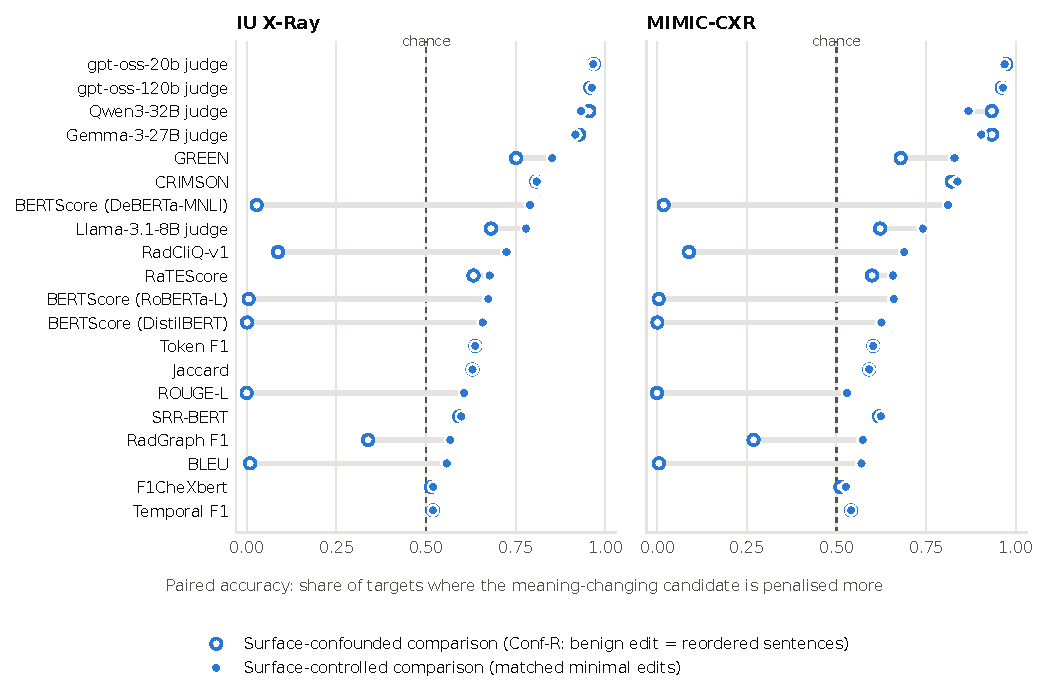
\includegraphics[width=\columnwidth]{figures/fig2_confound_vs_controlled.pdf}
\caption{Paired accuracy under a surface-confounded comparison (hollow; benign edit reorders sentences) and under the matched comparison (filled).}
\label{fig:dumbbell}
\end{figure}

\subsection{Meaning Sensitivity and Surface Sensitivity Are Separate Axes}

Figure~\ref{fig:scatter} places each metric by two standardised effects: the extra penalty for a meaning change at fixed surface (C0 $-$ P0) and the extra penalty for paraphrasing the context at fixed meaning (P2 $-$ P0). Three groups appear. For BLEU, ROUGE-L, BERTScore, RadGraph and RadCliQ, the surface effect is 1.4--2.1 standard deviations and the meaning effect at most 0.25. F1CheXbert, temporal F1 and RaTEScore react weakly to both. CRIMSON and the stronger judges have a meaning effect above 0.9 and a surface effect near zero; GREEN and Llama-3.1-8B combine a large meaning effect with a surface effect of 0.1--0.6.
The surface penalty of the first group grows with the amount rewritten, from about 0.9 standard deviations in the least rewritten quartile of P2 to 2.5--2.7 in the most rewritten (Appendix~\ref{app:dose}), while paired accuracy within S2 stays flat. Paraphrase therefore does not erase the meaning signal of these metrics; it adds a large offset that swamps it whenever the two candidates differ in how much they were rewritten. In a model with meaning, surface layer and their interaction, the interaction is within $\pm0.03$ for all metrics except GREEN ($-0.24$) and Llama-3.1-8B ($-0.22$).

\begin{figure}[t]
\centering
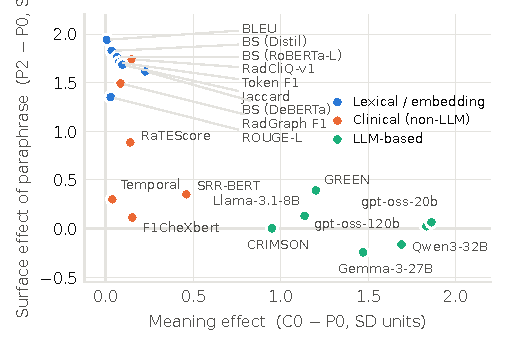
\includegraphics[width=\columnwidth]{figures/fig3_meaning_vs_surface.pdf}
\caption{Standardised penalty for a meaning change at fixed surface (x) against the penalty for paraphrasing the context at fixed meaning (y).}
\label{fig:scatter}
\end{figure}

\subsection{LLM Judges: Near Ceiling, With Specific Failures}

\begin{table*}[t]
\centering
\small
\setlength{\tabcolsep}{4.5pt}
\begin{adjustbox}{max width=\textwidth}
\begin{tabular}{lcccccccccccc}
\toprule
 & \multicolumn{6}{c}{\textbf{IU X-Ray}} & \multicolumn{6}{c}{\textbf{MIMIC-CXR}} \\
\cmidrule(lr){2-7}\cmidrule(lr){8-13}
 & \multicolumn{3}{c}{False alarms $\downarrow$} & \multicolumn{3}{c}{Detections $\uparrow$} & \multicolumn{3}{c}{False alarms $\downarrow$} & \multicolumn{3}{c}{Detections $\uparrow$} \\
\cmidrule(lr){2-4}\cmidrule(lr){5-7}\cmidrule(lr){8-10}\cmidrule(lr){11-13}
\textbf{Judge} & P0 & P1 & P2 & C0 & C1 & C2 & P0 & P1 & P2 & C0 & C1 & C2 \\
\midrule
Llama-3.1-8B & 0.17 & 0.58 & 0.25 & 0.69 & 0.88 & 0.71 & 0.15 & 0.59 & 0.25 & 0.61 & 0.85 & 0.66 \\
Gemma-3-27B & 0.21 & 0.24 & 0.09 & 0.93 & 0.90 & 0.84 & 0.29 & 0.31 & 0.10 & 0.94 & 0.88 & 0.81 \\
Qwen3-32B & 0.11 & 0.06 & 0.02 & 0.93 & 0.86 & 0.83 & 0.26 & 0.17 & 0.11 & 0.94 & 0.84 & 0.82 \\
Qwen3-32B (thinking) & 0.03 & 0.02 & 0.03 & 0.96 & 0.96 & 0.95 & 0.06 & 0.06 & 0.06 & 0.98 & 0.97 & 0.97 \\
gpt-oss-20b & 0.03 & 0.03 & 0.07 & 0.96 & 0.96 & 0.95 & 0.05 & 0.04 & 0.09 & 0.98 & 0.97 & 0.95 \\
gpt-oss-120b & 0.06 & 0.07 & 0.07 & 0.97 & 0.96 & 0.97 & 0.07 & 0.08 & 0.10 & 0.99 & 0.98 & 0.98 \\
\bottomrule
\end{tabular}
\end{adjustbox}
\caption{Share of candidates that a judge labels as meaning-changing (rubric prompt). Meaning-preserving cells should be near 0, meaning-changing cells near 1. Identity pairs are flagged in at most 0.6\% of cases for every judge.}
\label{tab:judges}
\end{table*}

The reasoning models are close to ceiling: gpt-oss-20b, gpt-oss-120b and Qwen3-32B with thinking reach 0.95--0.97 in both controlled comparisons (Table~\ref{tab:main}), and unlike most metrics the judges are not hurt by the confounded comparisons, since a visibly rewritten benign candidate is easy to accept. Matched minimal pairs are thus not out of reach for current LLMs, and it is the controlled comparison, not the confounded one, that is harder for them. The remaining errors are structured (Table~\ref{tab:judges}; by type in Appendix~\ref{app:judges}).

\textbf{Matched benign edits still trigger false alarms.} Gemma-3-27B flags 22--29\% of P0 candidates and Qwen3-32B without thinking 11--26\%, concentrated in unit conversions (``4.7 cm'' $\to$ ``47 mm'' is called a change by Gemma in 85--87\% of cases, and by Qwen3 in 96\% on MIMIC-CXR, where most measurements describe device positions) and in severity synonyms. Over-penalisation of harmless rewrites by LLM judges \citep{beyond-scalar-2026} is therefore not only an effect of rewrite size.

\textbf{Sentence order matters for a small model.} Llama-3.1-8B flags 58--59\% of reordered benign candidates (P1) against 15--17\% of P0.

\textbf{Certainty changes are missed under paraphrase.} When the context is paraphrased, a flipped hedge (``may represent'' $\leftrightarrow$ ``represents'') is detected in only 29--40\% of cases by Gemma-3-27B, Qwen3-32B and Llama-3.1-8B, against 82--93\% without paraphrase for the first two; the reasoning models reach 68--90\%. The S2 layer acts as a harder tier of the same test.

\textbf{The prompt can matter more than the model.} With the errors prompt, Gemma-3-27B lists at least one ``discrepancy'' for 90--99\% of meaning-preserving candidates and its \ctrlt paired accuracy falls from 0.93 to 0.34; Qwen3-32B falls from 0.92 to 0.87, while both gpt-oss models stay at 0.93--0.96 (Appendix~\ref{app:prompt}).

\subsection{Monotonicity at Fixed Surface}

\begin{table}[t]
\centering
\scriptsize
\setlength{\tabcolsep}{2.5pt}
\begin{adjustbox}{max width=\columnwidth}
\begin{tabular}{lccccccc}
\toprule
 & \multicolumn{4}{c}{\textbf{Fixed-surface ladder}} & \multicolumn{2}{c}{\textbf{Growing-surface ladder}} & \textbf{3 benign} \\
\cmidrule(lr){2-5}\cmidrule(lr){6-7}
\textbf{Metric} & $\tau$ & $0{\to}1$ & $1{\to}2$ & $2{\to}3$ & $1{\to}2$ & $2{\to}3$ & \textbf{$>$ 1 error} \\
\midrule
\multicolumn{8}{l}{\textit{Meaning-blind baselines}} \\
Jaccard & 0.41 & 0.60 & 0.61 & 0.63 & 0.99 & 0.99 & 0.98 \\
Token F1 & 0.46 & 0.61 & 0.62 & 0.64 & 1.00 & 1.00 & 1.00 \\
\addlinespace[2pt]
\multicolumn{8}{l}{\textit{Lexical / embedding}} \\
BLEU & 0.17 & 0.53 & 0.53 & 0.55 & 1.00 & 1.00 & 1.00 \\
ROUGE-L & 0.36 & 0.58 & 0.58 & 0.59 & 1.00 & 1.00 & 1.00 \\
BERTScore (DistilBERT) & 0.36 & 0.72 & 0.66 & 0.65 & 1.00 & 1.00 & 1.00 \\
BERTScore (RoBERTa-L) & 0.56 & 0.78 & 0.78 & 0.69 & 1.00 & 0.99 & 0.99 \\
BERTScore (DeBERTa-MNLI) & 0.74 & 0.81 & 0.83 & 0.79 & 1.00 & 1.00 & 0.85 \\
\addlinespace[2pt]
\multicolumn{8}{l}{\textit{Clinical, non-LLM}} \\
F1CheXbert & 0.00 & 0.50 & 0.50 & 0.50 & 0.53 & 0.53 & 0.56 \\
Temporal F1 & 0.11 & 0.51 & 0.53 & 0.54 & 0.62 & 0.64 & 0.74 \\
SRR-BERT & 0.36 & 0.59 & 0.59 & 0.58 & 0.61 & 0.59 & 0.44 \\
RadGraph F1 & 0.16 & 0.57 & 0.55 & 0.49 & 0.95 & 0.96 & 0.96 \\
RaTEScore & 0.48 & 0.71 & 0.72 & 0.70 & 0.95 & 0.96 & 0.88 \\
RadCliQ-v1 & 0.58 & 0.74 & 0.77 & 0.71 & 1.00 & 0.99 & 0.97 \\
\addlinespace[2pt]
\multicolumn{8}{l}{\textit{LLM-based metrics}} \\
GREEN & 0.77 & 0.76 & 0.77 & 0.74 & 0.85 & 0.85 & 0.34 \\
CRIMSON & 0.88 & 0.86 & 0.83 & 0.85 & 0.83 & 0.85 & 0.15 \\
\addlinespace[2pt]
\multicolumn{8}{l}{\textit{LLM judges (rubric prompt)}} \\
Llama-3.1-8B & 0.46 & 0.68 & 0.60 & 0.54 & 0.60 & 0.50 & 0.34 \\
Gemma-3-27B & 0.58 & 0.87 & 0.59 & 0.54 & 0.44 & 0.42 & 0.05 \\
Qwen3-32B & 0.64 & 0.88 & 0.61 & 0.57 & 0.42 & 0.48 & 0.06 \\
Qwen3-32B (thinking) & 0.68 & 0.98 & 0.49 & 0.52 & 0.48 & 0.51 & 0.01 \\
gpt-oss-20b & 0.69 & 0.96 & 0.52 & 0.56 & 0.55 & 0.53 & 0.04 \\
gpt-oss-120b & 0.73 & 0.97 & 0.53 & 0.60 & 0.54 & 0.59 & 0.02 \\
\addlinespace[2pt]
\multicolumn{8}{l}{\textit{LLM judges (errors prompt)}} \\
Gemma-3-27B & 0.33 & 0.47 & 0.60 & 0.68 & 0.98 & 0.98 & 0.98 \\
Qwen3-32B & 0.73 & 0.77 & 0.73 & 0.77 & 0.97 & 0.97 & 0.46 \\
gpt-oss-20b & 0.96 & 0.91 & 0.93 & 0.93 & 0.99 & 0.99 & 0.19 \\
gpt-oss-120b & 0.98 & 0.96 & 0.97 & 0.97 & 0.99 & 0.99 & 0.06 \\
\bottomrule
\end{tabular}
\end{adjustbox}
\caption{Monotonicity on 300 MIMIC-CXR sections. \emph{Fixed-surface ladder}: all candidates edit the same three sites and contain 0--3 meaning changes; $\tau$ is the mean within-target Kendall correlation between the number of meaning changes and the penalty, and $i{\to}j$ the share of targets whose penalty increases from $i$ to $j$ changes. \emph{Growing-surface ladder}: each added error is also an added edit. Last column: share of targets where three benign edits are penalised more than one real error.}
\label{tab:mono}
\end{table}

Table~\ref{tab:mono} contrasts the two ladders of \S\ref{sec:monodesign}. On the growing-surface ladder BLEU, ROUGE-L, the BERTScore variants, RadCliQ, RadGraph and the meaning-blind baselines increase their penalty with every added error in 95--100\% of targets. On the fixed-surface ladder the same metrics have $\tau$ between 0.16 and 0.58 (BLEU 0.18, RadGraph 0.16, Jaccard 0.41), and each step is detected little better than by chance for BLEU, ROUGE-L and RadGraph. These metrics also penalise three harmless edits more than one real error in 96--100\% of targets. A monotonicity test in which errors and edits grow together therefore cannot distinguish a metric that counts errors from one that measures edit distance.

Under control, the two error-enumerating LLM metrics are the most monotone (CRIMSON $\tau{=}0.88$, GREEN 0.77). Rubric-style judges detect the first meaning change (0.87--0.98) but barely react to the second and third (0.52--0.61): a binary verdict with a confidence does not grade. Judges are the best classifiers of whether meaning changed, and enumeration-based metrics the better graders of how much.

\subsection{Edit Types}

Per-type results (Appendix~\ref{app:types}) refine known blind spots. (i) On \emph{severity}, BERTScore with DistilBERT, RadGraph and RadCliQ are below chance under control (0.07--0.38): replacing ``mild'' by ``slight'' is penalised more than replacing it by ``moderate''. LLM-based scorers show a dose--response, with extreme grade changes easier than adjacent ones. This result depends on the severity synonyms being accepted as meaning-preserving (\S\ref{sec:human}). (ii) On \emph{uncertainty}, GREEN and CRIMSON are near chance (0.54--0.57) while general-purpose judges reach 0.82--0.93. CRIMSON does recognise these edits: it assigns a certainty error to 91--96\% of them, but the error barely moves its score (Appendix~\ref{app:crimson}); the blindness lies in the weighting, not the detection. (iii) Label-based metrics are exactly at chance outside their label space.

\section{Discussion and Recommendations}

\paragraph{What a perturbation suite measures.}
A perturbation suite supports a claim about meaning only to the extent that its two classes cannot be told apart by surface form. That condition was not met by our earlier suite, and published averages suggest it is not met elsewhere. Because the direction of the artefact depends on the construction of benign edits, results from different suites are not comparable and can contradict each other for the same metric.

\paragraph{Two inexpensive controls.}
We recommend that perturbation-based meta-evaluations report (i) a \emph{meaning-blind baseline} such as Jaccard next to every metric, and (ii) a \emph{surface-only predictability} score for the labels. Both need no annotation and no GPU. A metric should be credited with semantic sensitivity only for what it achieves beyond the baseline on a set whose labels are not predictable from surface.

\paragraph{For metric users.}
Overlap, embedding and graph metrics are dominated by how much text was rewritten; their scores are informative about meaning only when systems phrase reports alike. Among non-judge metrics, CRIMSON is the most stable across surface conditions and GREEN the most sensitive to matched edits but affected by paraphrase. A strong LLM judge with a rubric prompt is the most accurate detector of a meaning change, at a higher cost and without grading; prompts that ask a weaker model to enumerate errors should be validated on meaning-preserving pairs first.

\section{Conclusion}

Separating surface from semantics changes what perturbation tests say about radiology report metrics: a reported reversal disappears, apparent monotonicity turns out to be edit distance, and several clinical metrics fall below a token-overlap baseline, while LLM-based scorers hold up with specific, reproducible failures. The design and both controls apply to any reference-based metric.

\section*{Limitations}

\bench tests a text-level property: whether a metric distinguishes a candidate that restates the reference from one that states something different. It does not assess correctness with respect to the image, and it makes no claim about clinical significance; we do not weight edit types by their consequences for patients. \tbd{Human validation is by two non-clinician annotators; no radiologist reviewed the substitution lexicon. Validation by clinicians is left to an extended version.}
Controlled comparisons are not perfectly surface-free: in \ctrlz the surface-only probe reaches 0.62--0.64 and Jaccard 0.59--0.63, because a flip removes the original token more often than a benign substitution does. We report the baseline and test against it instead of claiming a clean control. One measurement subtype (10-fold unit error) violates shape matching, since its \Pc edit changes two tokens and its \Cc edit one; it is reported separately and excluded in the robustness analysis. A few negation rewrites of telegraphic sentences are awkward.
Edits are local substitutions of seven types. Omissions and insertions of whole findings cannot be matched at a position; our attempt to control them at sentence level failed the surface probe (Appendix~\ref{app:oi}) and is not used for conclusions. Rule-based edits do not cover the distribution of errors made by generation systems.
S2 paraphrases are produced by an LLM of the Qwen family and accepted by an NLI model and lexical guards; residual meaning drift (e.g.\ ``large'' rendered as ``significant'') is possible and affects \Pc and \Cc of a target identically. One judge shares the paraphraser's model family.
The monotonicity set and the sentence-level layer exist only for MIMIC-CXR, as IU X-Ray sections are too short. RadEval's domain-adapted BERTScore could not be run in our environment. Results for proprietary judges are \tbd{pending}.

\section*{Ethical Considerations}

We use de-identified reports from IU X-Ray (public) and MIMIC-CXR (credentialed access). MIMIC-CXR text was processed only with locally hosted models and is not redistributed; we release code, rule tables, identifiers and reconstruction scripts for MIMIC-CXR, and pairs, scores and judge outputs for IU X-Ray. The benchmark evaluates metrics, not clinical systems; a metric that does well on it is not thereby validated for clinical use. \tbd{Annotator recruitment, compensation, consent, and ethics-review status.}

\bibliography{references}

\clearpage
\appendix

\section{Edit Rules}
\label{app:rules}

\begin{table*}[t]
\centering
\scriptsize
\setlength{\tabcolsep}{4pt}
\begin{tabular}{p{0.085\textwidth}p{0.25\textwidth}p{0.26\textwidth}p{0.26\textwidth}p{0.07\textwidth}}
\toprule
\textbf{Type} & \textbf{Trigger (exactly once in sentence and section)} & \textbf{\Pc: meaning-preserving} & \textbf{\Cc: meaning-changing} & \textbf{Subtypes} \\
\midrule
Laterality & \emph{left/right} + finding noun or lobe; no \emph{bilateral/both}; no device terms; not negated & \emph{left X} $\to$ \emph{left-sided X}; \emph{X on the left}; \emph{left lower lobe} $\to$ \emph{LLL} & same operation with the other side: \emph{right-sided X}; \emph{X on the right}; \emph{RLL} & -- \\
Region & side + lobe; \emph{lung bases}; side + \emph{(lung) base}; \emph{bibasilar}; \emph{basilar}; \emph{perihilar} & \emph{LLL}; \emph{bases of the lungs}; \emph{base of the left lung}; \emph{bilateral basilar}; \emph{basal}; \emph{parahilar} & \emph{LUL}; \emph{apices of the lungs}; \emph{apex of the left lung}; \emph{bilateral apical}; \emph{apical}; \emph{peripheral} & -- \\
Negation & \emph{No X is seen}; \emph{There is no X}; \emph{No X.}; \emph{without X}; \emph{no evidence of X}; \emph{negative for X}; \emph{X is seen} (X contains a finding term; no other negation cue) & \emph{No X seen} / \emph{No X is identified}; \emph{There is no evidence of X}; \emph{X is absent}; \emph{with no X}; \emph{no sign of X}; \emph{negative for any X}; \emph{X seen} / \emph{X is visualized} & \emph{X is seen}; \emph{There is evidence of X}; \emph{X is present}; \emph{with new X}; \emph{new evidence of X}; \emph{positive for X}; \emph{X not seen} / \emph{X is not seen} & negated$\to$present; present$\to$negated \\
Measurement & one number with \emph{cm/mm}, $0<v\le40$ & same quantity in the other unit: \emph{4.7 cm} $\to$ \emph{47 mm} & \emph{94 mm} (value $\times2$ or $\div2$) or \emph{47 cm} (10-fold error) & value; unit \\
Temporal & \emph{unchanged, stable, improved, worsened, has/have increased, decreased, resolved, new}; no device terms; no other comparison cue & \emph{stable} $\leftrightarrow$ \emph{unchanged}; \emph{better}; \emph{worse}; \emph{progressed}; \emph{diminished}; \emph{cleared}; \emph{newly identified} & direction reversed: \emph{increased/worsened/improved}; \emph{decreased}; \emph{persisted}; \emph{previously seen} & -- \\
Severity & \emph{trace, minimal, mild, small, moderate, large, severe, marked} modifying a finding; not negated & \emph{slight}; \emph{marked} $\leftrightarrow$ \emph{severe}; \emph{trace} $\leftrightarrow$ \emph{minimal}; \emph{small-sized}; \emph{moderate-sized}; \emph{large-volume} & another grade on the same scale & adjacent; extreme \\
Uncertainty & \emph{may/could represent, likely represents, possibly representing, cannot be excluded, suspicious for, suggestive of, questionable, probable, possible, consistent/compatible with, represents} & hedge of the same strength: \emph{might represent}; \emph{probably}; \emph{cannot be ruled out}; \emph{concerning for}; \emph{compatible} $\leftrightarrow$ \emph{consistent} & \emph{clearly represents}; \emph{is excluded}; \emph{consistent with}; \emph{definite}; or \emph{suspicious for}, \emph{may represent} & hedged$\to$definite; definite$\to$hedged \\
\bottomrule
\end{tabular}
\caption{Edit rules (abridged; the released code is authoritative). Every \Pc/\Cc pair is produced at the same position and must differ by at most one token in edit size.}
\label{tab:rules}
\end{table*}

Table~\ref{tab:rules} lists the rules. Rules are deterministic given a seed derived from the report identifier.

\section{Set Composition}
\label{app:sets}

\begin{table*}[t]
\centering
\small
\begin{adjustbox}{max width=\textwidth}
\begin{tabular}{lrrrrrrrrrrr}
\toprule
\textbf{Corpus} & \textbf{Targets} & \textbf{Reports} & Anat. & Lat. & Meas. & Neg. & Sev. & Temp. & Unc. & \textbf{Patterns} & \textbf{Para.\ acc.\ (\%)} \\
\midrule
IU X-Ray & 890 & 714 & 150 & 146 & 94 & 119 & 137 & 150 & 94 & 47 & 91.9 \\
MIMIC-CXR & 1,050 & 1,037 & 150 & 150 & 150 & 150 & 150 & 150 & 150 & 64 & 92.2 \\
\bottomrule
\end{tabular}
\end{adjustbox}
\caption{Composition of the factorial sets. Each target yields an identity pair and six candidates. \emph{Patterns}: number of distinct rewrite patterns. \emph{Para.\ acc.}: share of context sentences with an accepted paraphrase in S2.}
\label{tab:sets}
\end{table*}

Table~\ref{tab:sets} gives counts per edit type. The monotonicity set has 300 MIMIC-CXR targets and seven candidates each.

\section{Results by Edit Type}
\label{app:types}

\begin{table*}[t]
\centering
\small
\begin{adjustbox}{max width=\textwidth}
\begin{tabular}{lccccccc}
\toprule
\textbf{Metric} & Anat. & Lat. & Meas. & Neg. & Sev. & Temp. & Unc. \\
\midrule
\multicolumn{8}{l}{\textit{Meaning-blind baselines}} \\
Jaccard & 0.65 & 0.75 & 0.32 & 0.58 & 0.73 & 0.54 & 0.78 \\
Token F1 & 0.66 & 0.76 & 0.32 & 0.67 & 0.74 & 0.50 & 0.77 \\
\multicolumn{8}{l}{\textit{Lexical / embedding}} \\
BLEU & 0.64 & 0.51 & 0.24 & 0.73 & 0.50 & 0.50 & 0.77 \\
ROUGE-L & 0.50 & 0.74 & 0.32 & 0.67 & 0.74 & 0.50 & 0.74 \\
BERTScore (DistilBERT) & 0.81 & 0.80 & 0.41 & 0.74 & 0.07 & 0.91 & 0.80 \\
BERTScore (RoBERTa-L) & 0.83 & 0.79 & 0.33 & 0.87 & 0.23 & 0.81 & 0.78 \\
BERTScore (DeBERTa-MNLI) & 0.93 & 0.79 & 0.50 & 1.00 & 0.51 & 0.87 & 0.87 \\
\multicolumn{8}{l}{\textit{Clinical, non-LLM}} \\
F1CheXbert & 0.50 & 0.50 & 0.50 & 0.64 & 0.50 & 0.51 & 0.50 \\
Temporal F1 & 0.50 & 0.50 & 0.50 & 0.54 & 0.50 & 0.58 & 0.50 \\
SRR-BERT & 0.53 & 0.52 & 0.50 & 0.88 & 0.51 & 0.58 & 0.74 \\
RadGraph F1 & 0.63 & 0.52 & 0.46 & 0.85 & 0.33 & 0.50 & 0.74 \\
RaTEScore & 0.71 & 0.71 & 0.47 & 0.76 & 0.65 & 0.74 & 0.62 \\
RadCliQ-v1 & 0.91 & 0.76 & 0.45 & 0.95 & 0.35 & 0.77 & 0.83 \\
\multicolumn{8}{l}{\textit{LLM-based metrics}} \\
GREEN & 0.85 & 0.92 & 0.72 & 0.92 & 0.90 & 0.96 & 0.55 \\
CRIMSON & 0.87 & 0.88 & 0.73 & 0.94 & 0.89 & 0.72 & 0.54 \\
\multicolumn{8}{l}{\textit{LLM judges (rubric prompt)}} \\
Llama-3.1-8B & 0.68 & 0.77 & 0.65 & 0.96 & 0.84 & 0.86 & 0.62 \\
Gemma-3-27B & 0.95 & 0.94 & 0.58 & 0.99 & 0.94 & 0.99 & 0.93 \\
Qwen3-32B & 0.94 & 0.96 & 0.81 & 0.98 & 0.95 & 0.99 & 0.82 \\
Qwen3-32B (thinking) & 1.00 & 1.00 & 0.92 & 1.00 & 0.96 & 1.00 & 0.88 \\
gpt-oss-20b & 0.97 & 0.99 & 0.99 & 0.99 & 0.92 & 1.00 & 0.89 \\
gpt-oss-120b & 1.00 & 1.00 & 0.82 & 0.99 & 0.97 & 1.00 & 0.89 \\
\bottomrule
\end{tabular}
\end{adjustbox}
\caption{\ctrlz paired accuracy by edit type, IU X-Ray.}
\label{tab:typesiu}
\end{table*}

\begin{table*}[t]
\centering
\small
\begin{adjustbox}{max width=\textwidth}
\begin{tabular}{lccccccc}
\toprule
\textbf{Metric} & Anat. & Lat. & Meas. & Neg. & Sev. & Temp. & Unc. \\
\midrule
\multicolumn{8}{l}{\textit{Meaning-blind baselines}} \\
Jaccard & 0.66 & 0.83 & 0.25 & 0.53 & 0.68 & 0.48 & 0.71 \\
Token F1 & 0.67 & 0.83 & 0.24 & 0.56 & 0.72 & 0.50 & 0.70 \\
\multicolumn{8}{l}{\textit{Lexical / embedding}} \\
BLEU & 0.66 & 0.67 & 0.26 & 0.71 & 0.50 & 0.50 & 0.70 \\
ROUGE-L & 0.50 & 0.67 & 0.24 & 0.56 & 0.72 & 0.50 & 0.52 \\
BERTScore (DistilBERT) & 0.86 & 0.85 & 0.37 & 0.75 & 0.12 & 0.61 & 0.82 \\
BERTScore (RoBERTa-L) & 0.91 & 0.81 & 0.28 & 0.87 & 0.25 & 0.68 & 0.83 \\
BERTScore (DeBERTa-MNLI) & 0.91 & 0.81 & 0.49 & 1.00 & 0.58 & 0.98 & 0.90 \\
\multicolumn{8}{l}{\textit{Clinical, non-LLM}} \\
F1CheXbert & 0.50 & 0.50 & 0.50 & 0.64 & 0.50 & 0.53 & 0.51 \\
Temporal F1 & 0.50 & 0.50 & 0.50 & 0.58 & 0.50 & 0.70 & 0.50 \\
SRR-BERT & 0.53 & 0.50 & 0.50 & 0.93 & 0.51 & 0.62 & 0.78 \\
RadGraph F1 & 0.58 & 0.61 & 0.44 & 0.83 & 0.38 & 0.52 & 0.65 \\
RaTEScore & 0.73 & 0.72 & 0.43 & 0.83 & 0.63 & 0.63 & 0.63 \\
RadCliQ-v1 & 0.95 & 0.87 & 0.40 & 0.98 & 0.31 & 0.51 & 0.80 \\
\multicolumn{8}{l}{\textit{LLM-based metrics}} \\
GREEN & 0.83 & 0.92 & 0.82 & 0.95 & 0.82 & 0.91 & 0.55 \\
CRIMSON & 0.92 & 0.94 & 0.72 & 0.93 & 0.89 & 0.89 & 0.57 \\
\multicolumn{8}{l}{\textit{LLM judges (rubric prompt)}} \\
Llama-3.1-8B & 0.65 & 0.75 & 0.66 & 0.96 & 0.72 & 0.87 & 0.58 \\
Gemma-3-27B & 0.91 & 0.96 & 0.72 & 1.00 & 0.85 & 0.97 & 0.92 \\
Qwen3-32B & 0.92 & 0.95 & 0.54 & 0.99 & 0.89 & 0.94 & 0.85 \\
Qwen3-32B (thinking) & 1.00 & 1.00 & 0.82 & 0.99 & 0.96 & 0.99 & 0.97 \\
gpt-oss-20b & 0.97 & 0.99 & 0.98 & 0.99 & 0.92 & 0.99 & 0.94 \\
gpt-oss-120b & 1.00 & 1.00 & 0.87 & 0.99 & 0.95 & 1.00 & 0.95 \\
\bottomrule
\end{tabular}
\end{adjustbox}
\caption{\ctrlz paired accuracy by edit type, MIMIC-CXR.}
\label{tab:typesmimic}
\end{table*}

\begin{table*}[t]
\centering
\small
\begin{adjustbox}{max width=\textwidth}
\begin{tabular}{lcccccc}
\toprule
 & \multicolumn{2}{c}{\textbf{Severity}} & \multicolumn{2}{c}{\textbf{Measurement}} & \multicolumn{2}{c}{\textbf{Uncertainty}} \\
\cmidrule(lr){2-3}\cmidrule(lr){4-5}\cmidrule(lr){6-7}
\textbf{Metric} & adjacent & extreme & value & unit$^{\ddagger}$ & hedged$\to$def. & def.$\to$hedged \\
\midrule
\multicolumn{7}{l}{\textit{Meaning-blind baselines}} \\
Jaccard & 0.71/0.72 & 0.76/0.63 & 0.67/0.49 & 0.01/0.01 & 0.62/0.65 & 0.97/0.92 \\
Token F1 & 0.72/0.76 & 0.76/0.68 & 0.67/0.47 & 0.01/0.01 & 0.57/0.62 & 1.00/0.98 \\
\multicolumn{7}{l}{\textit{Lexical / embedding}} \\
BLEU & 0.50/0.50 & 0.50/0.50 & 0.50/0.50 & 0.01/0.01 & 0.57/0.62 & 1.00/0.98 \\
ROUGE-L & 0.72/0.76 & 0.76/0.68 & 0.67/0.47 & 0.01/0.01 & 0.55/0.52 & 0.98/0.53 \\
BERTScore (DistilBERT) & 0.00/0.08 & 0.14/0.16 & 0.87/0.75 & 0.00/0.00 & 0.63/0.77 & 1.00/1.00 \\
BERTScore (RoBERTa-L) & 0.21/0.19 & 0.26/0.32 & 0.67/0.55 & 0.02/0.01 & 0.78/0.83 & 0.77/0.82 \\
BERTScore (DeBERTa-MNLI) & 0.32/0.36 & 0.72/0.79 & 0.62/0.69 & 0.39/0.29 & 0.76/0.90 & 1.00/0.91 \\
\multicolumn{7}{l}{\textit{Clinical, non-LLM}} \\
F1CheXbert & 0.50/0.51 & 0.50/0.49 & 0.50/0.50 & 0.50/0.50 & 0.50/0.50 & 0.50/0.52 \\
Temporal F1 & 0.50/0.50 & 0.50/0.50 & 0.50/0.50 & 0.50/0.50 & 0.50/0.50 & 0.50/0.50 \\
SRR-BERT & 0.51/0.51 & 0.52/0.52 & 0.50/0.50 & 0.50/0.49 & 0.71/0.75 & 0.78/0.86 \\
RadGraph F1 & 0.33/0.30 & 0.33/0.45 & 0.43/0.49 & 0.49/0.39 & 0.67/0.62 & 0.84/0.79 \\
RaTEScore & 0.56/0.53 & 0.74/0.74 & 0.78/0.60 & 0.19/0.25 & 0.65/0.67 & 0.59/0.52 \\
RadCliQ-v1 & 0.31/0.28 & 0.40/0.34 & 0.76/0.69 & 0.16/0.11 & 0.71/0.79 & 0.98/0.85 \\
\multicolumn{7}{l}{\textit{LLM-based metrics}} \\
GREEN & 0.83/0.82 & 0.98/0.82 & 0.81/0.80 & 0.64/0.84 & 0.56/0.57 & 0.55/0.50 \\
CRIMSON & 0.81/0.83 & 0.98/0.95 & 0.72/0.77 & 0.74/0.67 & 0.58/0.59 & 0.50/0.50 \\
\multicolumn{7}{l}{\textit{LLM judges (rubric prompt)}} \\
Llama-3.1-8B & 0.76/0.64 & 0.92/0.80 & 0.57/0.52 & 0.73/0.79 & 0.61/0.59 & 0.64/0.58 \\
Gemma-3-27B & 0.90/0.81 & 0.98/0.89 & 0.54/0.74 & 0.61/0.69 & 0.89/0.94 & 0.98/0.86 \\
Qwen3-32B & 0.92/0.88 & 0.99/0.89 & 0.80/0.53 & 0.82/0.54 & 0.84/0.90 & 0.80/0.70 \\
Qwen3-32B (thinking) & 0.93/0.94 & 0.98/0.97 & 0.93/0.83 & 0.91/0.80 & 0.90/0.97 & 0.85/0.94 \\
gpt-oss-20b & 0.90/0.91 & 0.93/0.93 & 1.00/0.99 & 0.99/0.97 & 0.87/0.93 & 0.92/0.98 \\
gpt-oss-120b & 0.94/0.95 & 0.99/0.95 & 0.87/0.86 & 0.79/0.88 & 0.90/0.96 & 0.87/0.91 \\
\bottomrule
\end{tabular}
\end{adjustbox}
\caption{\ctrlz paired accuracy by subtype (IU X-Ray / MIMIC-CXR). $^{\ddagger}$The unit subtype is not shape-matched (the \Pc edit changes two tokens, the \Cc edit one) and behaves like a confounded comparison for surface-driven metrics.}
\label{tab:subtypes}
\end{table*}

Tables~\ref{tab:typesiu}--\ref{tab:subtypes} give paired accuracy by type and subtype.

\section{Robustness to Flagged Edits}
\label{app:robust}

\begin{table*}[t]
\centering
\small
\begin{adjustbox}{max width=\textwidth}
\begin{tabular}{lcccc}
\toprule
\textbf{Metric} & All & $-$ unit subtype & $-$ flagged lexicon & $-$ all flagged \\
$n$ (IU/MIMIC) & 890/1050 & 841/975 & 724/854 & 673/773 \\
\midrule
\multicolumn{5}{l}{\textit{Meaning-blind baselines}} \\
Jaccard & 0.63/0.59 & 0.67/0.64 & 0.62/0.57 & 0.66/0.62 \\
Token F1 & 0.64/0.60 & 0.67/0.65 & 0.63/0.58 & 0.68/0.64 \\
\multicolumn{5}{l}{\textit{Lexical / embedding}} \\
BLEU & 0.56/0.57 & 0.59/0.61 & 0.58/0.58 & 0.62/0.63 \\
ROUGE-L & 0.61/0.53 & 0.64/0.57 & 0.58/0.50 & 0.62/0.55 \\
BERTScore (DistilBERT) & 0.66/0.63 & 0.70/0.67 & 0.73/0.67 & 0.79/0.73 \\
BERTScore (RoBERTa-L) & 0.67/0.66 & 0.71/0.71 & 0.75/0.71 & 0.81/0.77 \\
BERTScore (DeBERTa-MNLI) & 0.79/0.81 & 0.81/0.85 & 0.83/0.85 & 0.86/0.90 \\
\multicolumn{5}{l}{\textit{Clinical, non-LLM}} \\
F1CheXbert & 0.52/0.53 & 0.52/0.53 & 0.52/0.53 & 0.53/0.53 \\
Temporal F1 & 0.52/0.54 & 0.52/0.54 & 0.52/0.55 & 0.53/0.56 \\
SRR-BERT & 0.60/0.62 & 0.60/0.63 & 0.61/0.63 & 0.62/0.64 \\
RadGraph F1 & 0.57/0.57 & 0.57/0.59 & 0.60/0.61 & 0.61/0.63 \\
RaTEScore & 0.68/0.66 & 0.71/0.69 & 0.68/0.67 & 0.72/0.71 \\
RadCliQ-v1 & 0.72/0.69 & 0.76/0.73 & 0.77/0.72 & 0.82/0.77 \\
\multicolumn{5}{l}{\textit{LLM-based metrics}} \\
GREEN & 0.85/0.83 & 0.86/0.83 & 0.85/0.83 & 0.87/0.84 \\
CRIMSON & 0.81/0.84 & 0.81/0.85 & 0.80/0.84 & 0.81/0.86 \\
\multicolumn{5}{l}{\textit{LLM judges (rubric prompt)}} \\
Llama-3.1-8B & 0.78/0.74 & 0.78/0.74 & 0.78/0.75 & 0.79/0.75 \\
Gemma-3-27B & 0.92/0.90 & 0.93/0.92 & 0.91/0.91 & 0.94/0.93 \\
Qwen3-32B & 0.93/0.87 & 0.94/0.89 & 0.94/0.87 & 0.95/0.90 \\
Qwen3-32B (thinking) & 0.97/0.96 & 0.97/0.97 & 0.98/0.96 & 0.98/0.97 \\
gpt-oss-20b & 0.97/0.97 & 0.97/0.97 & 0.98/0.97 & 0.98/0.97 \\
gpt-oss-120b & 0.96/0.96 & 0.97/0.97 & 0.97/0.97 & 0.98/0.97 \\
\bottomrule
\end{tabular}
\end{adjustbox}
\caption{\ctrlz paired accuracy (IU X-Ray / MIMIC-CXR) on all targets and after removing, in turn, the non-matched unit subtype, every target whose meaning-preserving substitution we flagged in advance as debatable, and both together with eight awkward negation rewrites.}
\label{tab:robust}
\end{table*}

Table~\ref{tab:robust} shows that the conclusions of \S6.1 hold on the conservative subset; embedding-based metrics gain 0.07--0.13 when flagged substitutions are removed.

\section{Decomposition and Dose--Response}
\label{app:dose}

\begin{table*}[t]
\centering
\small
\begin{adjustbox}{max width=\textwidth}
\begin{tabular}{lccccccc}
\toprule
 & \multicolumn{5}{c}{\textbf{Standardised effects}} & \multicolumn{2}{c}{\textbf{Exchange rate}} \\
\cmidrule(lr){2-6}\cmidrule(lr){7-8}
\textbf{Metric} & Meaning (C0$-$P0) & Surface S1 (P1$-$P0) & Surface S2 (P2$-$P0) & Meaning@S2 (C2$-$P2) & Interaction S2 & reorder & paraphrase \\
\midrule
\multicolumn{8}{l}{\textit{Meaning-blind baselines}} \\
Jaccard & 0.10/0.05 & 0.00/0.00 & 1.68/1.88 & 0.07/0.03 & -0.02/-0.01 & 0.0/0.0 & 18/39 \\
Token F1 & 0.08/0.05 & 0.00/0.00 & 1.71/1.88 & 0.07/0.04 & -0.00/-0.00 & 0.0/0.0 & 22/42 \\
\multicolumn{8}{l}{\textit{Lexical / embedding}} \\
BLEU & 0.01/0.01 & 0.35/0.23 & 1.94/2.04 & 0.01/0.00 & -0.00/-0.00 & 51/33 & 282/284 \\
ROUGE-L & 0.03/0.01 & 2.00/2.00 & 1.35/1.58 & 0.03/0.01 & -0.00/0.00 & 70/298 & 47/235 \\
BERTScore (DistilBERT) & 0.03/0.02 & 1.19/1.23 & 1.83/2.06 & 0.04/0.02 & 0.00/-0.00 & 34/65 & 53/109 \\
BERTScore (RoBERTa-L) & 0.06/0.05 & 1.43/1.34 & 1.76/2.02 & 0.06/0.05 & -0.00/-0.00 & 22/28 & 27/42 \\
BERTScore (DeBERTa-MNLI) & 0.23/0.22 & 1.54/1.50 & 1.62/1.93 & 0.20/0.18 & -0.03/-0.04 & 6.8/6.9 & 7.1/9.0 \\
\multicolumn{8}{l}{\textit{Clinical, non-LLM}} \\
F1CheXbert & 0.15/0.19 & 0.04/0.10 & 0.11/0.22 & 0.14/0.22 & -0.02/0.03 & 0.2/0.5 & 0.8/1.2 \\
Temporal F1 & 0.04/0.08 & 0.00/0.00 & 0.30/0.72 & 0.04/0.05 & -0.00/-0.02 & 0.0/0.0 & 8.0/9.2 \\
SRR-BERT & 0.46/0.54 & 0.02/0.02 & 0.35/0.54 & 0.44/0.51 & -0.02/-0.03 & 0.0/0.0 & 0.8/1.0 \\
RadGraph F1 & 0.09/0.09 & 0.30/0.43 & 1.49/1.73 & 0.09/0.09 & 0.00/-0.01 & 3.5/4.7 & 18/19 \\
RaTEScore & 0.14/0.11 & 0.11/0.10 & 0.89/1.41 & 0.14/0.11 & 0.00/0.00 & 0.8/1.0 & 6.3/13 \\
RadCliQ-v1 & 0.15/0.15 & 0.76/0.81 & 1.74/1.99 & 0.13/0.15 & -0.02/-0.01 & 5.1/5.3 & 12/13 \\
\multicolumn{8}{l}{\textit{LLM-based metrics}} \\
GREEN & 1.20/1.03 & 0.26/0.30 & 0.39/0.59 & 0.96/0.93 & -0.24/-0.10 & 0.2/0.3 & 0.3/0.6 \\
CRIMSON & 0.95/0.87 & 0.00/0.03 & 0.00/0.01 & 0.92/0.83 & -0.03/-0.04 & 0.0/0.0 & 0.0/0.0 \\
\multicolumn{8}{l}{\textit{LLM judges (rubric prompt)}} \\
Llama-3.1-8B & 1.14/1.01 & 0.63/0.65 & 0.13/0.16 & 0.92/0.81 & -0.22/-0.19 & 0.6/0.6 & 0.1/0.2 \\
Gemma-3-27B & 1.47/1.35 & 0.04/0.02 & -0.24/-0.38 & 1.48/1.40 & 0.01/0.05 & 0.0/0.0 & -0.2/-0.3 \\
Qwen3-32B & 1.69/1.40 & -0.09/-0.18 & -0.16/-0.31 & 1.58/1.39 & -0.10/-0.01 & -0.1/-0.1 & -0.1/-0.2 \\
Qwen3-32B (thinking) & 1.86/1.83 & -0.02/-0.02 & -0.00/-0.03 & 1.84/1.83 & -0.02/-0.00 & -0.0/-0.0 & -0.0/-0.0 \\
gpt-oss-20b & 1.86/1.86 & -0.01/-0.02 & 0.06/0.08 & 1.77/1.73 & -0.09/-0.13 & -0.0/-0.0 & 0.0/0.0 \\
gpt-oss-120b & 1.83/1.84 & 0.02/0.01 & 0.02/0.06 & 1.80/1.77 & -0.03/-0.07 & 0.0/0.0 & 0.0/0.0 \\
\bottomrule
\end{tabular}
\end{adjustbox}
\caption{Standardised effects (IU X-Ray / MIMIC-CXR).}
\label{tab:decomp}
\end{table*}

\begin{figure*}[t]
\centering
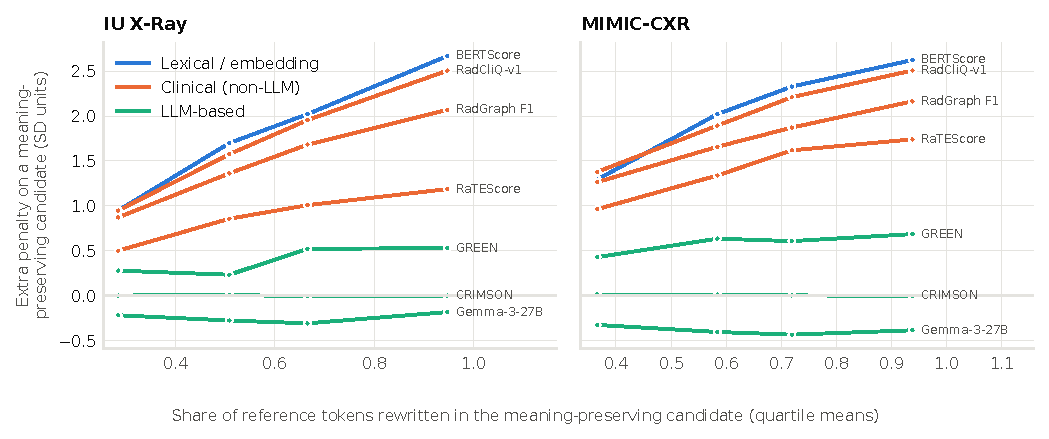
\includegraphics[width=0.8\textwidth]{figures/fig_dose_response.pdf}
\caption{Extra penalty on the meaning-preserving candidate P2 relative to P0, by quartile of the share of reference tokens rewritten.}
\label{fig:dose}
\end{figure*}

\section{LLM Judges by Edit Type and Prompt}
\label{app:judges}
\label{app:prompt}

\begin{table*}[t]
\centering
\small
\begin{adjustbox}{max width=\textwidth}
\begin{tabular}{lcccccccc}
\toprule
 & \multicolumn{4}{c}{\textbf{IU X-Ray}} & \multicolumn{4}{c}{\textbf{MIMIC-CXR}} \\
\cmidrule(lr){2-5}\cmidrule(lr){6-9}
 & \multicolumn{2}{c}{P0 false alarm $\downarrow$} & \multicolumn{2}{c}{C2 detection $\uparrow$} & \multicolumn{2}{c}{P0 false alarm $\downarrow$} & \multicolumn{2}{c}{C2 detection $\uparrow$} \\
\cmidrule(lr){2-3}\cmidrule(lr){4-5}\cmidrule(lr){6-7}\cmidrule(lr){8-9}
\textbf{Judge} & Meas. & Sev. & Unc. & Lat. & Meas. & Sev. & Unc. & Lat. \\
\midrule
Llama-3.1-8B & 0.84 & 0.14 & 0.37 & 0.58 & 0.48 & 0.13 & 0.40 & 0.55 \\
Gemma-3-27B & 0.87 & 0.34 & 0.34 & 0.73 & 0.85 & 0.54 & 0.39 & 0.71 \\
Qwen3-32B & 0.27 & 0.20 & 0.29 & 0.84 & 0.96 & 0.32 & 0.37 & 0.84 \\
Qwen3-32B (thinking) & 0.13 & 0.04 & 0.68 & 0.99 & 0.33 & 0.07 & 0.87 & 1.00 \\
gpt-oss-20b & 0.01 & 0.12 & 0.78 & 0.94 & 0.04 & 0.12 & 0.79 & 0.99 \\
gpt-oss-120b & 0.41 & 0.06 & 0.76 & 1.00 & 0.29 & 0.08 & 0.90 & 0.99 \\
\bottomrule
\end{tabular}
\end{adjustbox}
\caption{Selected type-level rates for the rubric prompt: false alarms on matched benign edits (P0) for measurement and severity; detections under paraphrase (C2) for uncertainty and laterality.}
\label{tab:judgestypes}
\end{table*}

\begin{table*}[t]
\centering
\small
\begin{adjustbox}{max width=\textwidth}
\begin{tabular}{llcccccc}
\toprule
 & & \multicolumn{3}{c}{\textbf{Paired accuracy}} & \multicolumn{3}{c}{\textbf{Rate flagged}} \\
\cmidrule(lr){3-5}\cmidrule(lr){6-8}
\textbf{Judge} & \textbf{Prompt} & \textsc{Ctrl-0} & \textsc{Ctrl-2} & \textsc{Conf-P} & P0 $\downarrow$ & P2 $\downarrow$ & C2 $\uparrow$ \\
\midrule
Gemma-3-27B & rubric & 0.92 & 0.93 & 0.96 & 0.21 & 0.09 & 0.84 \\
Gemma-3-27B & errors & 0.55 & 0.34 & 0.07 & 0.90 & 0.99 & 1.00 \\
Qwen3-32B & rubric & 0.93 & 0.91 & 0.96 & 0.11 & 0.02 & 0.83 \\
Qwen3-32B & errors & 0.88 & 0.87 & 0.82 & 0.20 & 0.24 & 0.95 \\
gpt-oss-20b & rubric & 0.97 & 0.96 & 0.96 & 0.03 & 0.07 & 0.95 \\
gpt-oss-20b & errors & 0.94 & 0.93 & 0.91 & 0.11 & 0.16 & 0.97 \\
gpt-oss-120b & rubric & 0.96 & 0.97 & 0.97 & 0.06 & 0.07 & 0.97 \\
gpt-oss-120b & errors & 0.97 & 0.96 & 0.95 & 0.05 & 0.08 & 0.98 \\
\bottomrule
\end{tabular}
\end{adjustbox}
\caption{Prompt sensitivity on IU X-Ray. For the errors prompt a candidate counts as flagged if at least one discrepancy is listed.}
\label{tab:prompt}
\end{table*}

\section{Error Attribution by CRIMSON}
\label{app:crimson}

\begin{table*}[t]
\centering
\small
\begin{adjustbox}{max width=\textwidth}
\begin{tabular}{llcccc}
\toprule
\textbf{Edit type} & \textbf{Expected category} & C0: any error & C0: expected cat. & P0: any error & Score paired acc. \\
\midrule
Anatomy & location & 0.95/0.97 & 0.94/0.97 & 0.11/0.09 & 0.87/0.92 \\
Laterality & location & 0.92/0.93 & 0.91/0.93 & 0.05/0.01 & 0.88/0.94 \\
Measurement & measurement & 0.96/0.85 & 0.95/0.83 & 0.63/0.70 & 0.73/0.72 \\
Negation & false/missing finding & 0.95/0.91 & 0.92/0.86 & 0.00/0.01 & 0.94/0.93 \\
Severity & severity & 0.99/1.00 & 0.99/0.99 & 0.52/0.54 & 0.89/0.89 \\
Temporal & temporal & 0.67/0.84 & 0.45/0.65 & 0.13/0.05 & 0.72/0.89 \\
Uncertainty & certainty & 0.98/0.92 & 0.96/0.91 & 0.52/0.49 & 0.54/0.57 \\
\bottomrule
\end{tabular}
\end{adjustbox}
\caption{CRIMSON error categories (IU X-Ray / MIMIC-CXR): share of candidates with at least one listed error, with an error of the expected category, and the paired accuracy of the final score.}
\label{tab:crimson}
\end{table*}

\section{A Sentence-Level Layer That Failed the Surface Probe}
\label{app:oi}

\begin{table}[t]
\centering
\small
\begin{adjustbox}{max width=\columnwidth}
\begin{tabular}{lcccc}
\toprule
 & \multicolumn{2}{c}{\textsc{Ctrl-0}} & \multicolumn{2}{c}{\textsc{Ctrl-2}} \\
\cmidrule(lr){2-3}\cmidrule(lr){4-5}
\textbf{Metric} & Omission & Insertion & Omission & Insertion \\
\midrule
\textit{Surface-only classifier (AUROC)} & 0.95 & 0.99 & 0.75 & 0.81 \\
\midrule
Jaccard & 0.67 & 0.99 & 0.69 & 0.98 \\
Token F1 & 0.75 & 0.50 & 0.78 & 0.53 \\
BLEU & 0.68 & 0.48 & 0.76 & 0.52 \\
ROUGE-L & 0.75 & 0.50 & 0.73 & 0.54 \\
BERTScore (DistilBERT) & 0.44 & 0.79 & 0.61 & 0.71 \\
BERTScore (RoBERTa-L) & 0.46 & 0.65 & 0.61 & 0.68 \\
BERTScore (DeBERTa-MNLI) & 0.78 & 0.04 & 0.73 & 0.04 \\
F1CheXbert & 0.84 & 0.76 & 0.84 & 0.74 \\
Temporal F1 & 0.63 & 0.51 & 0.64 & 0.53 \\
SRR-BERT & 0.91 & 0.96 & 0.89 & 0.96 \\
RadGraph F1 & 0.51 & 0.85 & 0.67 & 0.86 \\
RaTEScore & 0.93 & 0.92 & 0.92 & 0.95 \\
RadCliQ-v1 & 0.94 & 0.96 & 0.98 & 0.96 \\
GREEN & 0.98 & 0.90 & 0.81 & 0.89 \\
CRIMSON & 0.97 & 0.90 & 0.96 & 0.91 \\
Llama-3.1-8B & 0.75 & 0.63 & 0.65 & 0.74 \\
Gemma-3-27B & 0.78 & 0.98 & 0.78 & 0.91 \\
Qwen3-32B & 0.89 & 0.83 & 0.74 & 0.95 \\
gpt-oss-20b & 0.92 & 0.97 & 0.96 & 0.95 \\
gpt-oss-120b & 0.85 & 0.99 & 0.91 & 0.97 \\
\bottomrule
\end{tabular}
\end{adjustbox}
\caption{Omission/insertion layer (MIMIC-CXR, 150 targets each). The surface-only probe separates the classes, so paired accuracies are not controlled measurements.}
\label{tab:oi}
\end{table}

We attempted to extend the design to omitted and inserted findings by matching sentence-level operations: deleting a finding sentence vs.\ deleting a technique or comparison sentence, and appending a finding sentence from another report vs.\ appending a paraphrase of an existing sentence. The surface-only probe reaches 0.89 in the minimal layer (Table~\ref{tab:oi}), mainly because a restatement shares tokens with the report whereas a foreign sentence does not. We report the layer as a negative example of why the probe should be run before results are interpreted.

\section{Prompts and Implementation}
\label{app:prompts}

\paragraph{Rubric prompt.} The judge sees the reference and the candidate and is asked whether the candidate states exactly the same clinical findings; differences in wording, order, formatting, abbreviations and synonyms are to be treated as not changing the meaning, and changes in presence, laterality, location, severity or size, certainty, measurement or comparison as changing it. It answers with a JSON object containing a label (\textsc{preserved}/\textsc{changed}) and an integer confidence; the score is the confidence for \textsc{preserved} and one minus the confidence for \textsc{changed}.

\paragraph{Errors prompt.} The judge lists every clinically meaningful discrepancy, one per line, and ends with a line giving the count $n$; the score is $1/(1+n)$.

\paragraph{Decoding.} Temperature 0. For reasoning models only the final channel is parsed; outputs without a final answer (at most 0.5\% of rubric and 0.5\% of errors outputs) are treated as missing.

\paragraph{Software.} RadEval 2.2.1, bert-score 0.3.13, green-score 0.0.12, vLLM 0.30. GREEN uses RadLlama2-7B; CRIMSON uses the released MedGemma-4B checkpoint with the reference prompt and scoring code, with batched generation.

\paragraph{Human annotation.} \tbd{Instructions, annotator background, time, agreement tables.}

\end{document}
